\chapter{Heaps}

\section{Heaps}\label{sec:Heaps}

We can now discuss a visual representation of Coxeter group elements. Each reduced expression can be associated with a labeled partially ordered set (poset) called a heap.  Heaps provide a visual representation of a reduced expression while preserving the relations among the generators. We follow the development of heaps of straight line Coxeter groups in~\cite{Billey2007},~\cite{Ernst2010}, and~\cite{Stembridge1996}. 

Let $(W,S)$ be a Coxeter system of type $\Gamma$. Suppose $\overline{w}=s_{x_1}s_{x_2}\cdots s_{x_r}$ is a fixed reduced expression for $w \in W$. As in~\cite{Stembridge1996}, we define a partial ordering on the indices $\{1, 2, \ldots, r\}$ by the transitive closure of the relation $\lessdot$ defined via $j \lessdot i$ if $i < j$ and $s_{x_i}$ and $s_{x_j}$ do not commute. In particular, since $\overline{w}$ is reduced, $j \lessdot i$ if $s_{x_i}=s_{x_j}$ by transitivity. This partial order is referred to as the \emph{heap} of $\overline{w}$, where $i$ is labeled by $s_{x_i}$. Note that for simplicity we are omitting the labels of the underlying poset but retaining the labels of the corresponding generators.

It follows from~\cite{Stembridge1996} that heaps are well-defined up to commutation class. That is, given two reduced expressions $\overline{w}$ and $\overline{w'}$ for $w \in W$ that are in the same commutation class, then the heaps for $\overline{w}$ and $\overline{w'}$ will be equal. In particular, if $w \in \FC(\Gamma)$, then $w$ has a one commutation class, and thus $w$ has a unique heap.

When $w$ is $\FC$, we wish to make a canonical choice for the representation of $H(w)$ by assembling the entries in a particular way. To do so, we position all of the entries corresponding to elements in $\mathcal{L}(w)$ in the same vertical position, and all of the remaining elements should be positioned as high as possible in the lattice point representation. For example, the representation in Figure~\ref{fig:FC heap} is the canonical representation for $w$. Note that our canonical representation of heaps corresponds to Cartier-Foata normal form for monomials~\cite{Cartier1969, Green2006a}. There are potentially many ways to illustrate a heap of an arbitrary reduced expression, each differing by the vertical placement of the blocks. For example, we can place blocks in vertical positions as high as possible, as low as possible, or some combination of low/high. In this thesis, we choose what we view to be the best representation of the heap for each example and when illustrating the heaps of arbitrary reduced expressions we will discuss the relative position of the entries but never the absolute coordinates. 

\begin{example}
Let $\overline{w}=s_1s_0s_4s_1s_3s_5s_2s_4s_6$ be a reduced expression for $w \in \FC(\widetilde{C}_6).$ We see that $\overline{w}$ is indexed by $\{1,2,3,4,5,6,7,8,9\}$. As an example, $1 \lessdot 0$ since $0 <1$ and $s_0$ and $s_1$ do not commute. The labeled Hasse diagram for the heap poset is seen in Figure~\ref{fig:Hasse}.
\begin{figure}[h]
\centering
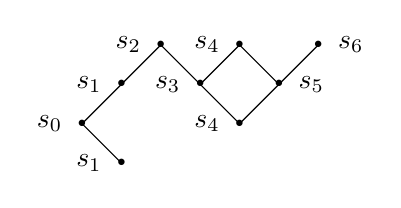
\begin{tikzpicture}[scale=0.5]
	\node[scale=0.6, label=left:$s_{2}$] at (2,5.5) {$\bullet$};
	\node[scale=0.6, label=left:$s_{4}$] at (4,5.5) {$\bullet$};
	\node[scale=0.6, label=right:$s_{6}$] at (6,5.5) {$\bullet$};
	\node[scale=0.6, label=left:$s_{1}$] at (1,4.5) {$\bullet$};
	\node[scale=0.6, label=left:$s_{3}$] at (3,4.5) {$\bullet$};
	\node[scale=0.6, label=right:$s_{5}$] at (5,4.5) {$\bullet$};
	\node[scale=0.6, label=left:$s_{0}$] at (0,3.5) {$\bullet$};
	\node[scale=0.6, label=left:$s_{4}$] at(4,3.5) {$\bullet$};
	\node[scale=0.6, label=left:$s_{1}$] at (1,2.5) {$\bullet$};
\draw (1,2.5)--(0,3.5)--(1,4.5)--(2,5.5)--(3,4.5)--(4,3.5);
\draw (3,4.5)--(4,5.5)--(5,4.5)--(4,3.5);
\draw (6,5.5)--(5,4.5);
\end{tikzpicture}
\caption{Labeled hasse diagram for the heap of an element in $\FC(\widetilde{C}_n)$}
\label{fig:Hasse}	
\end{figure}
\end{example}

Let $\overline{w}$ be a reduced expression for an element in $w \in W(\widetilde{C}_n)$. As in~\cite{Billey2007} and~\cite{Ernst2010} we can represent a heap for $\overline{w}$ as a set of lattice points embedded in $\{0,1,2,\ldots, n\} \times \mathbb{N}$. To do so, we assign coordinates (not unique) $(x,y) \in \{0,1,2,\ldots, n\} \times \mathbb{N}$ to each entry of the labeled Hasse diagram for the heap of $\overline{w}$ in such a way that:
\begin{enumerate}
\item An entry with coordinates $(x,y)$ is labeled $s_i$ (or $i$) in the heap if and only if $x = i$; 

\item If an entry with coordinates $(x,y)$ is greater than an entry with coordinates $(x',y')$ in the heap then $y > y'$.
\end{enumerate}

Although the above is specific to $W(\widetilde{C}_n)$, the same construction works for any straight line Coxeter graph with the appropriate adjustments made to the label set and assignments of coordinates. Specifically for type $A_n$ our label set is $\{1,2, \ldots, n\}~\times~\mathbb{N}$ and for type $B_n$ our label set is $\{0,1, \ldots, n-1\} \times \mathbb{N}$.

In the case of any straight line Coxeter graph it follows from the definition that $(x,y)$ covers $(x',y')$ in the heap if and only if $x = x' \pm 1$, $y > y'$, and there are no entries $(x'', y'')$ such that $x'' \in \{x, x'\}$ and $y'< y'' < y$. This implies that we can completely reconstruct the edges of the Hasse diagram and the corresponding heap poset from a lattice point representation. The lattice point representation can help us visualize arguments that are potentially complex. Note that in our heaps the entries in the top correspond to the generators occurring in the right descent set of the corresponding reduced expression.

Let $\overline{w}$ be a reduced expression for $w \in W(\widetilde{C}_n)$. We denote the lattice representation of the heap poset in $\{0,1,2, \ldots n\} \times n$ described in the preceding paragraphs via $H(\overline{w})$. If $w$ is $\FC$, then the choice of reduced expression for $w$ is irrelevant and we will often write $H(w)$ (note the absence of \textsf{sans serif} font) and we refer to $H(w)$ as the heap of $w$. As above the necessary adjustments to the lattice representation will result in a general result for heaps of all straight line coxeter graphs.

Given a heap, there are many possible coordinate assignments, yet the $x$-coordinates will be fixed for each entry will be fixed for all of them. In particular, two entries labeled by the same generator will only differ by the amount of vertical space between them while they will maintain the same horizontal position to adjacent entries in the heap.

Let $\overline{w}=s_{x_1}s_{x_2}\cdots s_{x_r}$ be a reduced expression for $w \in W(\widetilde{C}_n)$. If $s_{x_i}$ and $s_{x_j}$ are adjacent generators in the Coxeter graph with $i<j$, then we must place the point labeled by $s_{x_j}$ at a level that is \emph{above} the level of the point labeled by $s_{x_i}$. Because generators in a Coxeter graph that are not adjacent do commute, points whose $x$-coordinates differ more than one can slide past each other or land in the same level. To emphasize the covering relations of the lattice point representation we will enclose each entry in the heap in a square with rounded corners in such a way that if one entry covers another the squares overlap halfway. In addition, we will also label each square with $i$ representing the generator $s_i$.

\begin{example}
	Let $\overline{w}=s_1s_0s_4s_1s_3s_5s_2s_4s_6$ be a reduced expression for $w \in \FC(\widetilde{C}_6)$ as seen in Example 1.4.1. Figure~\ref{fig:FC heap} shows a possible lattice point representation for $H(w)$.
\begin{figure}[h]
\centering
\begin{tikzpicture}[scale=0.4]
\heapblock{2}{6}{2}{purple}
\heapblock{4}{6}{4}{purple}
\heapblock{6}{6}{6}{purple}
\heapblock{1}{4}{1}{purple}
\heapblock{3}{4}{3}{purple}
\heapblock{5}{4}{5}{purple}
\heapblock{0}{2}{0}{purple}
\heapblock{4}{2}{4}{purple}
\heapblock{1}{0}{1}{purple}
\end{tikzpicture}
\caption{A possible lattice point representation of for the heap of an FC element in $W(\widetilde{C}_6)$.}
\label{fig:FC heap}
\end{figure}
\end{example}

\begin{example}
Let $\overline{w}_1=s_1s_2s_3s_4s_2s_0$ be a reduced expression for $w \in W(\widetilde{C}_4)$. Applying the commutation $s_4s_2=s_2s_4$, we can obtain another reduced expression for $w$, namely $\overline{w}_2$ which is in the same commutation class as $\overline{w_1}$ and hence has the same heap. However, applying the braid move $s_2s_3s_2=s_3s_2s_3$, we obtain another reduced expression $\overline{w_3}=s_1s_3s_2s_3s_4s_0$. Note that since $\overline{w}_3$ was obtained by applying a braid move, $\overline{w_3}$ is in a different commutation class than $\overline{w_1}$ and $\overline{w_2}$. Representations of $H(\overline{w}_1), H(\overline{w}_2)$ and $H(\overline{w_3})$ are seen in Figure~\ref{fig:not FC} where the braid relation is colored in orange.

\begin{figure}[h]
\centering
\begin{subfigure}[b]{0.3\textwidth}	
\centering
\begin{tikzpicture}[scale=0.4]
\heapblock{0}{6}{0}{purple}
\heapblock{2}{6}{2}{orange}
\heapblock{4}{6}{4}{purple}	
\heapblock{3}{4}{3}{orange}
\heapblock{2}{2}{2}{orange}
\heapblock{1}{0}{1}{purple}
\end{tikzpicture}
\caption{$H(\overline{w}_1)$ and $H(\overline{w}_2)$ in $W(\widetilde{C}_4$.}
\end{subfigure}
\begin{subfigure}[b]{0.3\textwidth}	
\centering
\begin{tikzpicture}[scale=0.4]
\heapblock{10}{6}{0}{purple}
\heapblock{14}{6}{4}{purple}
\heapblock{13}{4}{3}{orange}
\heapblock{12}{2}{2}{orange}
\heapblock{11}{0}{1}{purple}
\heapblock{13}{0}{3}{orange}
\end{tikzpicture}
\caption{$H(\overline{w}_3)$}
\end{subfigure}
\caption{Two heaps of a non-FC element}	
\label{fig:not FC}
\end{figure}
\end{example}



